% simulations
We use simulations to provide additional evidence for theoretical claims and gain insight into audit behavior. As in \cite{sims}, we use margins from the 2020 US Presidential election, state-wide pairwise margins between the leading two candidates of 5\% or more. Narrower margins are computationally expensive, especially for the simulations with an underyling tie which quickly increase in sample size. We use the simulator in the R2B2 software library\cite{r2b2}. We perform $10000=10^4$ trials per margin for both an underyling outcomed as announced and an underyling tie.

\begin{figure}
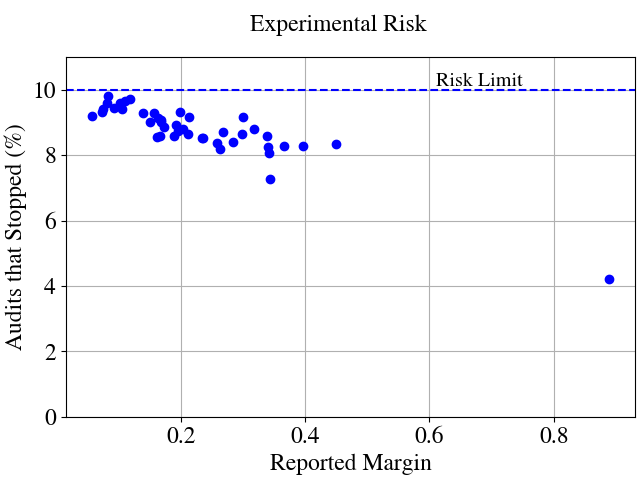
\includegraphics[width=.5\textwidth]{prov_risk.png}
\caption{The percent of simulated audits \Providence with an underlying tie that stopped in any of the five simulated rounds. This percent gives an estimate of the risk of the \Providence.}
\label{fig:prov-risk}
\end{figure}

In the simulations with an underlying tie, the percent of audits that stop, as shown in Figure~\ref{fig:prov-risk}, give an estimate of maximum risk. For all margins, this estimated risk is less than the risk limit, supporting the claim that \Providence is risk-limiting.

\begin{figure}
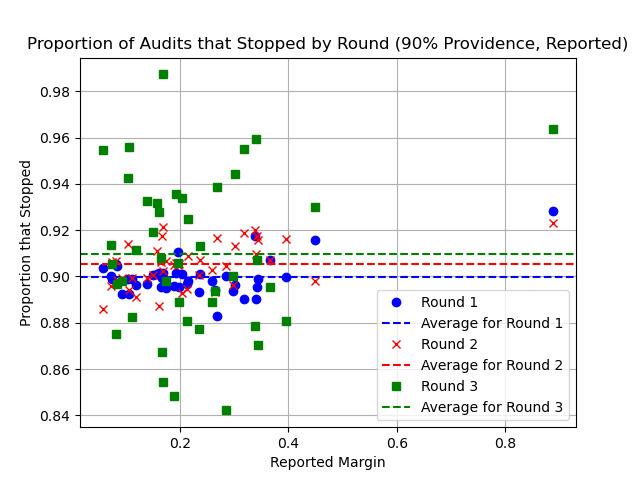
\includegraphics[width=.5\textwidth]{prov_sprob.png}
\caption{For the simulated \Providence audits with underlying margin as announced, the percent of audits that stopped among those that entered a round. This percent gives an estimate of the stopping probability conditioned on the sample of the previous round. The average percent for rounds 1, 2, and 3 is $89.96\%$, $90.52\%$, and $90.98\%$ respectively. We show only the first three rounds since so few audits make it to rounds 4 and 5.}
\label{fig:prov-sprob}
\end{figure}

Simulations with the underlying ballot distribution as announced provide insight into stopping probability and number of ballots drawn. Figure~\ref{fig:prov-sprob} shows that the stoping probabilities over the first rounds are near and slightly above $90\%$ as expected since our software chose round sizes to give at least a $90\%$ conditional stopping probability.
Figure~\ref{fig:prov-asn} shows that the probability of stopping as a function of number of ballots sampled. Points above (higher probability of stopping) and to the left (fewer ballots) represent more efficient audits. As shown, \Providence has comparable efficiency to \Minerva, while both are significantly more efficient than either implementation of \BRAVO. Note that a difference in twice as many ballots could be negligible in a contest with a wide margin. In a contest with a narrow margin (in the 2020 US Presidential election, eight states had margins less than $3\%$) the difference in number of ballots sampled could be weeks of work. Section~\ref{sec:workload} discusses workload in more depth.

\begin{figure}
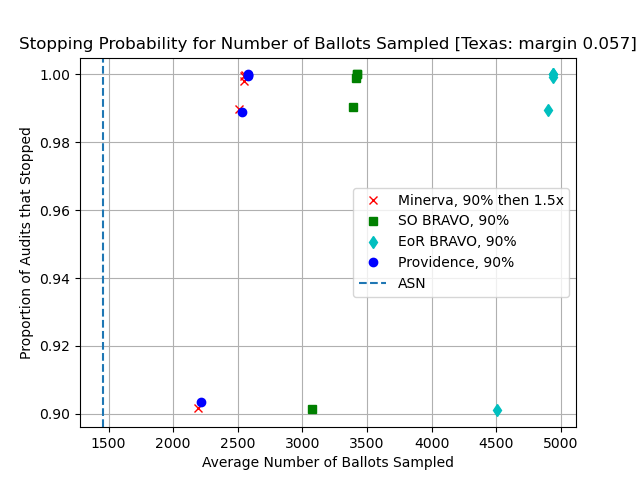
\includegraphics[width=.5\textwidth]{prov_asn.png}
\caption{For all five rounds, the estimated stopping probability for average number of ballots drawn for \Providence, \Minerva, EoR \BRAVO, and SO \BRAVO.}
\label{fig:prov-asn}
\end{figure}








